
%TODO må skrives: sett av 2 dager


%todo todo todo todo todo todo todo todo todo todo todo todo todo todo todo todo todo todo todo todo todo todo todo todo todo todo todo todo todo todo todo todo todo 
%
% 	ENDRE TITTEL til "comparison and discussion".      "comparison and discussion"       "comparison and discussion"       "comparison and discussion"       "comparison and discussion"       "comparison and discussion" 
% 		-> og endre tittel på neste kapittel til "Conclution"..
% 	Når kode/design skal sammenlignes: Gå gjennom, or fiks opp appendixDifferentDoTaskFunctions.tex 	Analysen skal være her, men de relevante doTask() funksjoner skal ligge der. No ligger alle der, og på norsk..
%
%todo todo todo todo todo todo todo todo todo todo todo todo todo todo todo todo todo todo todo todo todo todo todo todo todo todo todo todo todo todo todo todo todo 




% Sammenligning:
% Oppgave 3) Compare the new concept with competing methods. The evaluation may be based on a number of specific scenarios (with respect to input data etc.).
% 	Skriv at konkurerende metoder må tolkes til SANN, siden det blir for mykje å sammenligne med fANN også. Dette er en av styrkene til KANN: Kan snakke med alle!
% 	Skriv at for å kunne sammenligne med SANN, så har eg implementert begge. Dette gjør at eg kan meir grundig sammenligne implementering av de to. 
% 		Eg blir også bedre kjendt med implementasjonen så lettere å seinere gjennomføre en vilkensomhelst test (ikkje med rammer som er satt av implementasjonen).
%
% 	- Sammenligning om implementasjon OG kjøring om: Bra/dårlig ved:
% 		- implementasjon av de to
% 		- sensor(best for KANN)
% 		- Effektivitet (teoretisk sammenligning)
% 			- sammenligning av kva som krever ressurser:
% 				SANN: Generell input, lekkasje kvar iter, 
% 				KANN: endring av kappa er det tunge ( lekkasje er med i ligninga ) : bare når nødvendig.
% 						- hente ut verdien bare når den trengs. Koster bare når det er behov (ingen uptime keep).
% 						-osv. Dette er gøy å tenke på, men no: tilbake til arbeidet..
% 		- Sammenligning KANN vs SANN : heilt anna fokus for når nodene fyrer. For SANN har vi en reaktiv variant, der vi reagerer når noden går over terskel, for KANN har vi en proaktiv variant, som 
% 			beregner når den vil fyre, og bare ligger å venter på dette. 		--Her må man også diskutere/sjå på om dette er bedre for effektivitet. Ikkje heilt sikkert..
%
%
% 		- kjøretid (effektivitet for ulike 'scenarios') - DISKURS
% 		- over nettverk : best for KANN. 				- DISKURS
%


% - Sammenligning: Snakk om forskjellen i når aktivitetsVariabel propagates. Dette kan sikkert diskuteres mykje..



%Intro til kapittelet:
%	Intro: oppsummere kva som er gjort i dette prosjektet:
%		- Modellere neuronet.
%		- Utvikle KANN (som resultat av ligninene fra over)
%		- Utvikle SANN. Laga selv for best å kunne sammenligne forskjellene.
%		For begge ANN:  Sterk inspirert av biologien.
%			-> i tillegg til fordelane som er nevnt tidligare: gir eit felles design for implementasjonane av de to modellane => Meir sammenlignbar.
In this project two artificial neural networks have been designed and implemented. 
For the implementation it has been focused on comparability, both in respect to the design of the simulation and the behavior of the indivitual node.
The systems will be more comparable if both systems have the same blueprint. 
This is one of the reasons why the implementations are so inspired by biology.
An other cause for the strong resemblance with the biological neuron is the recognised connection between each generation of ANN; As ANN models evolve, each generation become closer to the biological version. %skriv om xxx.
This observation is a strong motivation of make the impementation close to the biological neuron, as long as it does not affect the effectivity of the simulator. %bruk fleire setninger?
%The comparability in design and implementation it the cause of an, in some cases, overly complicated object model.

For comparing the behavior of the indivitual nodes of the two nodels, some effort was put into a capabel logging system. 
Different elements of the node with interresting variables of effects were logged by this system. This includes the \emph{K\_synapse}, the \emph{K\_auron} and the \emph{s\_auron}.
The synapse is logged mainly for design purposes. The two auron elements were logged for design purposes and for the ``depolarization'' value comparison.
Both auron models is able to write the ``depolarization'' to a log file. The $\kappa$N is also able to log it's activity level, through $\kappa$.

The activity level of a spiking neuron us not formalized; Neuroscientist often use variables such as the firing frequency to measure the activity of a neuron.
For this reason, no method has been implemented for logging the activity level of the SANN nodes.
The activity of the single node is a phenomenon that first becomes important when we analyze larger neural networks.
For the comparison of the single node, the value of the node is the best comparison variable. 
%This containt more information, and if analyzed also contains information of the firing frequency and the synaptic input of the node could be found.
In this report it is most interresting with the transient depolarization curve of the nodes.




\section{Comparison of Design and Implementation for the Two Models}

	% Design av de to implementasjonane er gjordt som en direkte simulering av neuronet (spiking neurons), med dendrite, axon, osv. 
	% 	Dette førte til at eg begynte å impelmentere de to som like, bare med peiker-funksjoner for de funksjonane som trenkte å være ulike.
	% 	Eg oppdaga raskt at dette ikkje ville fungere, siden nesten alt er ulikt fra SANN til KANN.
	% 	Endte opp med å ha en interface class for kvart element (i_[element]) som arva til de to modellenes design av elementet (s_elemen og K_element).
	% 		Dette førte til at forskjellane i design ble veldig tydlige. Fellestrekka for de to modellane ble også veldig tydlige.
	% nevne det som står kommentert ut i section{Design for each node, ...} ?
	%
	% Nevn også at objektmodellen la opp designet (for begge modellimplementasjoner), og eg oppfatta først etterpå at dette kunne gjøres langt meir effektivt for KANN.
	%  

	%In this project, both implementations were designed to make the differences stand out.
	In this project, the implementation of the two models is designed to make the differences stand out. %stand out:dårlig
	The nodes were designed as the biological neuron, both to give a common design to both models and to make the design more recognizable for the reader with knowledge of neuroscience.
	All common aspects of the subelements of each node is placed in an abstract class derived to the model--specific classes.

	The abstract interface class is named \emph{i\_[element]}, and the model--specific class is named \emph{s\_[element]} for the SN and \emph{K\_[element]} for the $\kappa$N.
	Here \emph{[element]} can be one of the four elements each node consists of; The dendrite, the auron, the axon or the synapse.

	As the design made it possible to place all similarities for the two models in the common abstract \emph{i\_element} class, the similarities and differences between the models became prominent.
	%In this section some of the similarities between each element will be presented.
	
	In this section the results will be presented.  %TODO TODO TODO TODO TODO TODO TODO TODO TODO TODO TODO TODO  ENDRE avslutting av intro.
	The section will first and foremost be about the differences in design and implementation, but some other aspects can be found. % xxx xxx skriv om xxx xxx
	The section will start by a comparison the fundamental aspects on each model, before moving on with a comparison of the subelements of each node.
	%This will start by presenting a comparison between the individual elements before presenting a larger view of the differences between the models. % TODO Sjekk at dette er rett. Endre setning når section er skrevet..

	\subsection{The activity level}
	
	%The largest and most immediate difference between the two models is how the activity level is represented.
	The most immediate difference between the two models is how the activity level is represented.
	The SANN model is a direct simulation of the depolarization of the neuron. 
	Synaptic input alters the value of the node, 
	If the value goes above the firing threshold, a simulated action potential is fired.
	The value of the node is modelled as a leaky integration of the node's input, and each time iteration we have a little dissapation of the value.

	For the $\kappa$ANN model, use higher order mathemathics to calculate the firing time of the node.
	Each node is modelled as a LIF neuron, and the leaky integration is included in the equations used by $\kappa$ANN (sec. \ref{secMatematiskModelleringAvBioNeuron}).
	%In these equations we calculate the firing time of the node, given a constant level of input until firing of the node. 
	% %As the equations from sec. \sec{secMatematiskModelleringAvBioNeuron} requires a constant activity level, the concept of a time window wa s introduced.
	
	The activity variable of a $\kappa$N is based on the notion of the final value of the simulated depolarization value of the node.
	Given a constant level of input and a constant degree of leakage, the value of the node will converge to some value $\kappa$.

	As the variable sertainly will change before the end of some period, the concept of a time window was introduced.
	The concept of the time window enables the use the model in an artificial neural network, if the state of the node is updated each time the activation level is altered for the node.

	By the use of the value $\kappa$ and the concept of time windows, the values that is important for signal processing in the neuron can be calculated for the $\kappa$N.
	One important difference between the $\kappa$N and the SN is therefore the use of the activity variable.
	For the SN, the activity variable is used for a direct simulation of the neuron's value, or depolarization.
	A spike will occur when this value goes to suprathreshold levels.
	%This gives a reactive responce to the input spikes.
	%In $\kappa$ANN, each node times the next spike by using a forecast based on equations presented in sec. \ref{secMatematiskModelleringAvBioNeuron}. 
	In $\kappa$ANN, each node use a forecast for timing the spike.
	This estimated spike time is based on equations presented in sec. \ref{secMatematiskModelleringAvBioNeuron}. %TODO TODO SKRIV OM
	%The estimate is updated every time the activity variable is changed, and 
	When the estimated time is the same as the next time iteration, the element is inserted into \emph{pWorkTaskQue}.
	%MEIR XXX


	\subsection{Information propagation}
	Synaptic transmission can be said to give the transmission of the activity of one node to the next.
	As the activity variable of the node differs between the two models, synaptic transmission is also different for the two models.

	In a SN, the transmission directly alters the postsynaptic value of the node.
	As for every other aspect of SANN, synaptic transmission is a direct simulation of the relevant aspects of the biological equivalent.
	Thansmission through an excitatory synaptse thus increase the postsynaptic activation level and an inhibitory synaptic transmission decrease the postsynaptic activation level.

	For the $\kappa$N, the activation level is a consequence of the \emph{level} of input to the node.
	As the presynaptic node is capable of esmimating the future firing frequency of the node, synaptic transmission between two nodes is given by this frequency scaled by the synaptic weight.

	The activity variable of a $\kappa$N is a time--invariant variable, as the final value of the node does not dissapate with time;
		The final value of the node (from eq. \ref{eqKappaSomFinalValueAvV}) is constant over time, given a constant level of input.
	Each transmission is therefore time invariant, and the postsynaptic node's activity variable can be recalculated at any time.
	The postsynaptic activity level could therefore be calculated as the sum of all synaptic input transmissions after the transmissions in one input synapse is altered.

	For the sake of efficiancy, the edge transmission is defined.
	The edge transmission is defined as the change in the synaptic transmission.
	%For the sake of efficiancy, the concept of the edge transmission as the derived is used in this implementation.
	A new edge transmission thus only needs to be added to the postsynaptic activity variable at the time of transmission.
	%In this case the postsynaptic activity variable could be updated by adding the edge transmission to the postsynaptic activity variable.
	The strenght of the time invariant aspect of the signal become appearent when the activity variable $\kappa$ is recalculated to hinder a global trunctation errors.


%	In this section, some of the similarities and differences between each node element is presented.
%	The activity level of the two models differs tematically.
%	For a SN, the activity level corresponds to the simulated depolarization of the node, while for the $\kappa$N the activity level 

	%Meir

%XXX HOVEDFORSKJELL: SN : integrerer input for å få state. 		KN: Umiddelbart input gir state, sammen med input historie.
	
	\subsection{Comparison of the indivitual node elements}
	%	%todo SKRIV OM! Innledning til section
	%In this section, some of the similarities and differences between each element of a node will be presented.
	%
	%The result will be presented in the order the signal propagates through a node.
	% 	%First the difference in synaptic transmission will be presented.
	%We will start out by taking a look at the differences in synaptic tranmission; 
	%	What is transmitted and how the sigal affects the postsynaptic node.
	%When synaptic transmission for the two models has been introduced, the mechanisms of the signal propagation within each node will be discussed.
	% 	%As the mechanisms of the activity of each node differ strongly, the activity variable of each node is 
	% 	%The difference in the activity level of each node differs strongly, as a resu
	%This section will be concluded by listing the similarities between the two models. 
				
	As the elements of each node is designed by having a common abstract class derived to the two modes, the aspects that are different between the SN and the $\kappa$N stand out more clearly.
	The similar aspects between the models are represented in the common interface class.

	In this section, the differences in design for the indivitual elements of the two model--specific nodes are presented. %TODO Dårlig setning!
	The results are presented in the order of the signal propagation within each node.
	
	%XXX Skal dette være med? Skriv om!
	The comparison is presented in the order of the internal signal propagation within each node.
	We will start by discussing an incoming synaptic transmission, continue to the dendrite's responce, before discussing the differences in the auron's and the axon's responce.
	%The elements are compared by the function that defines the element's behaviour in time, the \emph{timeInterface} derived virtual function \emph{doTask()}.
	%As this is what defines the action of the node, the design of this implementation isolates the location of the differences between each model--specific element. %XXX BLABLA TODO Fullfør.
	% %First the mechanisms of signal transmission will be presented, by comparing the two synapse designs.
	% %The results for the difference in dendritic integration of all input synapses transmission will then be presented.

		\subsubsection{The Mechanisms of the Synapse Element}
		The activity variable of the two nodes and thus the model for synaptic transmission is fundamental different for the two models.
		%For the SN, the activity variable give the node's state compared to the firing threshold.  Synaptic input is inte
		In the SN, synaptic input is integrated to a ``depolarization'' for the node.
		When the value reach the firing threshold, an action potential is simulated in the node.
		For the $\kappa$N, the activity variable gives the \emph{level} of activity for the node, and the firing time is calulated from the present level of input.
		%In the SN, the activity variable gives the nodes charge towards the firing threshold.
		%For the $\kappa$N the activity variable gives the activity level of the node.
		%
		We therefore get that the mechanisms behind synaptic transmission is also fundamentally different, as this is what gives the next nodes activity variable. %is the input to the next node
		%
		This can be seen in the implementation of the two models' synapse functions. 
		A synaptic transmission is executed by the synapse's \emph{doTask()} function, and we can easily compare the mechanisms of the two.

		Synaptic transmission in the SANN model is implemented by simply adding the synaptic weight to the postsynaptic node's activity variable.
		%When the \emph{s\_synapse} executes a synaptic transmission, it adds the synaptic weight to the postsynaptic node's activation variable.
		%As stated in in section \ref{secSANN}, the SN is a direct simulation of the elements of the biological neuron.
		From sec. \ref{ssecTheSynapse}, we can see that this gives a direct simulation of synaptic transmission in the the biological synapse.
		%This can be seen if we compare the workings of the synaptic transmission in the \emph{s\_synapse} with the biological synapse, introduced in sec. \ref{ssecTheSynapse}.

		Synaptic transmission for the $\kappa$N is modelled in sec. \ref{ssecSynTransForANNliggeriKANNsection} by the presynaptic node's frequency and the synaptic weight.
		%For the $\kappa$N, synaptic transmission is defined in eq. \eqref{eqSynapticTransmissionForKANNimplementation} by the presynaptic node's frequency and the synaptic weight.
		The edge transmission is further defined as the change in synaptic transmission. % in this implementation.
		This gives that the postsynaptic activity variable can be updated by simply adding the edge transmission, and much redundant calculation is avoided.
		The resulting effects for the node is calculated once after the current time iteration.
		%When the postsynaptic node updates its activity variable, this is done by simply adding the edge transmission to its activity variable.

		% XXX SKRIV OM : We end up with the same transmission scheme, but the variables is 
		
		%TODO Skriv heilt om eller ta bort:
		%The code for the implementation of the two element's \emph{doTask()} function is included in appendix \ref{appendixDoTaskForSynapse}.
		%We can see the difference in synaptic transmission clearly from the code.

		%	%The above differences introduced in 
		The size of transmission in the $\kappa$N varies with the presynaptic period, further given by its activity variable.
		As the activity variable is given by the immediate input of the node, we get that the output transmission is given by the state and the present input of the node.
		It could therefore be said that the $\kappa$N is a Mealy automata of the biological neuron.
	
		%TODO Skrive at SN er en moore modell? (i forhold til siste linja over).

		%Skriv om tematisk forskjell: KN overfører variabel som eg gitt av nodens inputlevel..

		\subsubsection{The Mechanisms of the Dendrite Element}
		%Both the SN and the $\kappa$N is implemented as the derived of the postsynaptic activity variable.
		For both the SN and $\kappa$N, synaptic transmission gives the derived of the postsynaptic activity variable.
		The input to a node thus gives the same result \emph{for the activity variable} in a SN and a $\kappa$N.
		%For the activity variable, a new input therefore gives the same result for the $\kappa$N and the SN. 
		%Both \emph{newInputSignal(double)} adds the new input to the the activity variable.
		
		In SANN, the input is discarded if the node is in the state of being in a refraction period.
		The fist action of the \emph{s\_dendrite::doTask()} is therefore to see if the variable \emph{bBlockInput\_refractionTime} is set.
		%In SANN, the dendrite first has to see whether the postsynaptic node is in a refraction period. 
		If not, the dendrite starts to execute the algorithm of the postsynaptic part of synaptic tranmission.
		The leakage is calculated from eq. \eqref{eqLeakageForSANN}, before the synaptic input is added to the node's activity variable.
		%Prior to adding the new signal to the postsynaptic node's value, the dendrite calculates the leakage.
		%This is done by eq. \eqref{eqLeakageForSANN}. 

		As the postsynaptic node will fire an action potential as soon as the value of the node reaches threshold, 
			it is the task of \emph{newInputSignal(double)} to test this after the input is added to the node's value.
			%the \emph{newInputSignal(double)} function has to test this as a part of its algorithm. %the incmng signal transmission.
		The action potential is initiated after the predefined delay, implemented by serially linked internal node elements.
		If the delay is set to $n$ time iterations, the first element of a linked list of $n$ elements is inserted into \emph{pWorkTaskQue}.
		%If a delay is modelled into the simulation, the action potential is initiated after $n$ time steps, were $n$ is the predefined delay.
		%This is best done by letting the dendrite insert the first element in a linket list of $n$ elements into \emph{pWorkTaskQue}.

		For the $\kappa$N, the activity variable is time--invariant; From eq. \eqref{eqKappaSomFinalValueAvV} we get that $\kappa$ is the final value of the node, given a constant input.
		As $\kappa$ does not vary as a consequence of time alone, no calculation is needed for mechanisms like ``leakage''.
		The activity variable does not have to be compared to any threshold value or othervise tested.
		The only action needed after an edge transmission is adding the transmitted variable to the activity variable.
		%As $\kappa$ is time--invariant, nothing has to be calculated as a result to time alone. We can therefore effectively use an event--based simulation scheme.
		%This further gives that nothing has to be calculated as a function of time alone. 

		%By the scheme of edge transmission as the derived of the synaptic transmission, we can calculate the postsynaptic activity variable by simply adding the edge transmission.
		As the $\kappa$N calculates future firing time by the activity variable, we do not have to check the postsynaptic activity variable after each transmission.
		For the $\kappa$N, most of the operations of SN transmission is therefore avoided:
			%we therefore have that most of the operations for the SN dendrite input is avoided: 
		\begin{itemize}
			\item The leakage does not have to be calculated
			\item It is unnecessary to compare the activity variable to the firing threshold, or othervise evaluate $\kappa$ after each transmission.
			\item The simulation of intracellular transmission delay becomes obsolete. The delay can be included in the calculation of the firing time of the node.
			\item As firing is controlled by other mechanisms, no elements is inserted into \emph{pWorkTaskQue}
		\end{itemize}
		If we have a delay of $n$ time iterations before some element is to be executed, 
			$\kappa$ANN implements this by directly writing the planned task time to the element's \emph{ulEstimatedTaskTime\_for\_object} variable.
		%	$\kappa$ANN implements this by adding $n$ to the present time iterations and writing it to the elements \emph{ulEstimatedTaskTime\_for\_object} variable.
		%If a predefined delay of $n$ time steps is to be included in the simulation, in $\kappa$N this is done by directly adding $n$ to the estimated firing time of the node.
		%If a delay of $n$ time steps is defined before execution of some element task, in $\kappa$ANN this can ge done by directly writing the planned task time for that element 

%		If we take a look at the two \emph{newInputSignal(double)} functions, listed in appendix \ref{appendixNewInputSignalDendrite}, it can be noted that the $\kappa$N version is substantially smaller.
%		The size can, however be decieving, so we will now discuss the two functions.
%		%skriv om at calculateLeakage er stor operasjon. Med exp-funk
%		The SN dendrite calls the function \emph{calculateLeakage()} and the $\kappa$N calls the \emph{changeKappa\_derivedArg()} function.
%		The \emph{calculateLeakage()} function will calculate the leakage as a result of the time since the last calculation. 
%		This is doen by equation \eqref{eqLeakageForSANN}.
%		
%		For the $\kappa$N, dendrite calls the model--specific \emph{K\_auron::changeKappa(double)} function.
%		%This will be discussed in XXX SKal eg diskutere dette i auron?

		When we have an edge transmission in $\kappa$ANN, the dendrite calls the function \emph{K\_auron::changeKappa\_derivedArg(double)}. 
		For completeness, the code for this funcion is included here.
\begin{lstlisting}
inline void K_auron::changeKappa_derivedArg( double dInputDerived_arg)
{
	// add arg to Kappa
	dChangeInKappa_this_iter +=  dInputDerived_arg ;

	// Insert [this] pointer to pCalculationTaskQue
	time_class::addCalculationIn_pCalculatationTaskQue( this );

	writeKappaToLog();
}
\end{lstlisting}

		As we can see, the $\kappa$N uses the concept of \emph{pCalculatationTaskQue}, introduced in sec. \ref{ssecCalcultaionTaskQue}.
		Whenever $\kappa$ is changed, the node is scheduled for recalculation of all the values that is given by $\kappa$. %a new input changes $\kappa$, 
		Exampes of such variables is the firing frequency and the estimated firing time corresponding to the updated $\kappa$.
		%Exampes of this is the corresponding frequency to the present $\kappa$ and the estimated firing time. 
		When \emph{K\_auron::doCalculation()} is called, a new time window will be initialized, and	it is important that the activity variable is not changed before calculating the initial ``depolarization value'' for the new time window
			($v_0$ in eq. \ref{eqVerdiligninga}).
		The variable \emph{dChangeInKappa\_this\_iter} is used for collecting all changes in $\kappa$ for any time iteration.

		Due to the mechanisms of \emph{pCalculatationTaskQue}, the calculation of the above mentioned variables will only be executed once for any time iteration.
		%	this will only be done once for any time iteration.
		%
		% TODO VIKTIG Skriv at diskurs over gir at KN kalkuleres det meste bare en gang. For SANN sjekkes alt kvar gang vi har input.
		The difference in efficiancy between the two models will therefore depend on the number of inputs per time iteration.
		For the $\kappa$N we execute the heavy part of the calcutaion (at most) once every time iteration. 
		The other part of the work associated with an incoming transmission is only to add the edge transmission to the postsynaptic activity variable. 
		This is executed without any mentionable cost.
		%The other part of synaptic transmission is only to add the edge inputs to the postsynaptic activity variable, and is executed without any mentionable cost.

		For the SN, apart from the calculation of leakage, the amount of work will be constant for any incoming transmission.
		%For the SN, apart from the calculation of leakage, the same amount of work is done every time the node gets an incoming synaptic transmission.
		%Elements of this work is the general amount of actions, the three if--sentences that break up pipelining in the processor (there is also one inside the inlined function \emph{calculateLeakage()}).
		%
		This amount is given by two aspects, where the most important probably is the three if--sentences (two in the code listed in appendix \ref{appendixNewInputSignalDendrite} and one in the inlined function \emph{calculateLeakage()}).
		Each conditonal statement will break up the pipelining of the processor, and lead to a decrease in the efficiancy of the execution.

		\subsubsection{The Mechanisms of the Auron Element}
		In a direct simulation of the neuron, the auron has the role of every aspect that is close to the core of the neuron.
		Of the mechanisms of signal processing and propagation, only the initiation of the action potential is percieved as being important enough to simulate in the SN.
		The \emph{s\_auron::doTask()} therefore only have two tasks: inserting the auron's \emph{pOutputAxon} pointer into \emph{pWorkTaskQue} and resetting the activity variable (``depolarization'') to zero..
		The refraction period is started as soon as the value goes to suprathreshold levels, in \emph{s\_dendrite::newInputSignal(double)}. %XXX XXX  Skriv om: ref.p. er [starta]


%		The auron is the central element of each node, and contains the central mechanisms for signal propagation.
%		For the SN, this includes the depolarization variable (\emph{dAktivitetsVariabel}) and the time stamp used for the calculation or leakage. %og fyrin av AP.
%		For the $\kappa$N, this includes $\kappa$ (\emph{dAktivitetsVariabel}), the initial value for the depolarization and initial time iteration in the current time window and a variable containing the calculated period inverse.
%		The variable that contains the present period inverse is used for calculation of edge tranmission when $\kappa$ is changed.


% TODO XXX Dette er vel konklusjon?
		In $\kappa$ANN, the concept of task scheduling could be used to determine the time of execution for the individual elements of the node.
		This further removes the necessarity for multiple elements within each node; 
			Simulation of intracellular delay could then be executed more effectively by setting the task time of the interresting element directly.
		The concept of delay by simulation thus becomes obsolete, and we do not have to propagate the signal through the node.

		%If the auron is the only element of the $\kappa$N, it controls the central mechanisms
		In this implementation, the auron has the role of firing the action potential.
		When it fires an action potential, a new time window is initiated for the $\kappa$ equations.
		The \emph{dDepolAtStartOfTimeWindow} variable is set to zero, and the next planned task time is set to the present time plus the previously calculated period of the node.
		Action potential is propagated by the mechanisms used in SANN, but this is, as previously mentioned, unnecessary. 
		
%		The task of the $\kappa$N auron then to change the estimated task time for all the output elements and update the firing time of the node.
%		By updating the firing time, it is referred to the calculated period of the neuron. 
%		After firing, the estimation for the next firing time will be the present time iteration plus the calculated interspike period.
%
%		Examples of tasks that are to be executed after firing of the node is calculation of STDP of the node's synapses and transmission throught synapses going to output nodes of the SANN model.
%		Neither of these aspects have not been implemented in this project, but the mechanisms used by the $\kappa$N is easily implemented.

		As the $\kappa$N does not have to simulate the mechanisms behind the time delay, single--compartment implementation could be used to simulate a multiple--compartment model of the neuron.
		This is examplified in this impelementation, by letting the auron element be the only internal element of each node that requires the use of the \emph{doTask()} function.
		The synapse is in this context percieved as a element that lies between nodes, and is the only element apart from the auron that requires the use of the \emph{doTask()} function. %todo ikkje skriv "requires" igjen!
		As the simulated time delay scheme from the SANN model was used, the axon element had to use the \emph{doTask()} function.
		As soon as the above mentioned aspects was realized, the firing of a node without the use of an axon was tested.
		In this scheme, the estimated firing time was incresed by one (same as the axon time delay) and the code from \emph{K\_axon::doTask()} function was called directly from \emph{K\_auron::doTask()}.
		The result was identical, and it is concluded that this confirms the authors hypothesis about individual task planning for different elements.
		Further investigation of this mechanism was not conducted due to time constraints.
		%Further experimentation with this mechanism will have to be marked as further research. % XXX Eller noke
		
		%Skriv kvifor eg har brukt SANN design for KANN noden. 
		%This realization first came when this report was written. %(at eg kan bruke single-comp. imp.) %TODO skriv at eg realized dette først no.. XXX skriv ppå nytt. Dårlig framført..
		% Due to time constraints, the implementation will not be altered at this point. 
	
% xxx Ta med seinare, i seinare ovesiklig diskurs.
%xxx	As this implementation have been based on the SANN model, the \emph{K\_axon} also makes use of the \emph{doTask()} function.
%xxx	In this implementation, the \emph{K\_auron::doTask()} only calls the memberfunction \emph{doTransmission()}. This could as easily be called by a central element, or not at all. %For synapsene kan legges direkte inn som planl. oppg
%xxx	The alternative way of planning synaptic transmission and other planned tasks first became clear to the author durin the writing of this report, these aspects have not been implemented.
%xxx	As the principle of task planning has been used for the auron element, and can easily be extended to be used for other elements, this is included in the discussion.
		%The reasoning is sound, and the concept of estimated task time can easily be extended to synapses and other elements. Due to time constraints, this is unfortunately not implemented.
		

	

		\subsubsection{The Mechanisms of the Axon Element}
		The axon is where the difference in execution is most prominent.
		In absence of a suitable timing mechanism, the SN uses the axon as a pure time delay.
		At the time of firing for the node, the axon is inserted into \emph{pWorkTaskQue}.
		Let $n$ be the number of serially linked axon elements before some output synape.
		The synapse will now get a transmission after a delay of $n$ time iterations.
		We can therefore simulate the time delay before transmission at a particular synapse by the number of serially linked axon elements before it.

		For the $\kappa$N, the same result can be achieved by letting the $\kappa$N write the planned execution time to to the corresponding synapse in the $\kappa$ANN version of the network.
		The planned execution time for the synapse, $t_{e, syn}$ is given by
		\begin{equation}
			t_{e,syn} = t_f+n \qquad, \; \text{$t_f$ is the firing time of the node}
		\end{equation}
		If $t_{e, syn}$ is written to the corresponding synapse in the $\kappa$ANN, the synapse's \emph{doTask()} function is executed at the same time iteration as for the SN version of the network.
		%The same result it therefore achieved for the timing of the transmission in the $\kappa$N synapse as in the SN synapse, only with a much smaller effort for the simulator.
		The same result it therefore achieved for the time of transmission for the $\kappa$N synapse as for the SN synapse, only with a much smaller effort for the simulator.
																							% TODO Del opp setninga over, | HER, (over streken) ?







\section{Theoretical Comparison Between the two Models}
SKAL EG SKRIVE DETTE, her også? Sjå diskurs i conclution 1, neste fil.

%TODO TODO TODO TODO TODO TODO TODO TODO TODO TODO TODO TODO TODO TODO TODO TODO TODO TODO TODO TODO TODO TODO TODO TODO TODO TODO TODO TODO TODO TODO TODO TODO TODO TODO TODO TODO TODO TODO TODO TODO TODO TODO TODO TODO 
%TODO TODO TODO TODO TODO TODO TODO TODO TODO TODO TODO TODO TODO TODO TODO TODO TODO TODO TODO TODO TODO TODO TODO TODO TODO TODO TODO TODO TODO TODO TODO TODO TODO TODO TODO TODO TODO TODO TODO TODO TODO TODO TODO TODO 
%TODO TODO TODO TODO TODO TODO TODO TODO TODO TODO TODO TODO TODO TODO TODO TODO TODO TODO TODO TODO TODO TODO TODO TODO TODO TODO TODO TODO TODO TODO TODO TODO TODO TODO TODO TODO TODO TODO TODO TODO TODO TODO TODO TODO 
%TODO TODO TODO TODO TODO TODO TODO TODO TODO TODO TODO TODO TODO TODO TODO TODO TODO TODO TODO TODO TODO TODO TODO TODO TODO TODO TODO TODO TODO TODO TODO TODO TODO TODO TODO TODO TODO TODO TODO TODO TODO TODO TODO TODO 
(er her)..		



%%Viktig eksempel til diskurs.
%		In addition, we have the aspect of \emph{how} the activity of the node changes. 
%		Let us take an example where we simulate a neuron with a constant level of synaptic input.
%		For the $\kappa$N, the node will have a constant activity level, and does not have to recalculate the firing time of the node when the node fires.
%		When the node fires, the node writes the current time iteration plus the previously calculated period to the member variable \emph{ulEstimatedTaskTime\_for\_object}.
%		When the estimated task time is the same as \emph{time\_class::ulTime}, the node fires again and the same is repeated.
%		For the SN, the number of input transmissions stays at a constant level to produce the same firing frequency for the node.
%		The number of actions for the SN will therefore stay at a constant level throughtout the simulated period.
%		As the $\kappa$N only has to calculate its activity level initially in the example, when its $\kappa$ is changed, we get a large difference in work load for this example. 
%		
%		The example is unrealistic for most circuits, but it examplifies when $\kappa$ANN will be more effective than SANN.
%		Even thought the example is unrealistic, there might me situations where a $\kappa$N would be better than a SN.
%% TODO TODO TODO TODO TODO TODO TODO TODO TODO TODO TODO TODO TODO TODO TODO TODO TODO TODO TODO TODO TODO TODO 
%
%
%
%





\section{Comparison of The Mechanisms of the Elements}
\label{secComparisonOfMechanismsOfNodeElements}
	% XXX Dette skal hovedsaklig ligge i KANN, men siste plott skal også legges ved her (eller bare her?) \subsec.{Comparison between the transient time course of the depolarization of the K auron and s auron,Vettafaen kor det skal ligge}
	%\subsection{Comparison of the transient time course of nodes of the two models}
	\subsection{Transient Time Course of The Model--Specific Nodes}

%\section{Comparison between the transient time course of the depolarization of the K auron and s auron ,   Vettafaen kor det skal ligge}
To compare %the implementation of (?)
			the two models, the the first aspects to be compared is the depolarization  of a single node of each model.
%							we will start with comparing the depolarization of a single node from each model.
The same input to the two nodes should give the same transient time course of the nodes' depolarization.

Because of the complexity of the single node, we cannot use a network of neurons to generate an equal input to the analyzed neuron. 
At least not before we know that the two model--specific nodes give the same output. %TODO Skriv om. Litt.

% //{
%The solution for this problem is to design an own underclass K\_sensor\_auron for the $\kappa$ANN model and s\_sensor\_auron for the SANN model.
%Objects of these classes continously update its activity level by the output of some ``sensor function''.
% %This sensor function wa s designed to give an output appropriate for comparing the variants of the node.
%Both sensor classes are constructed by sending a function pointer into the constructor of the object. 
%The function sent in to the constructor as a function ponter could be specifically designed for the comparison in mind.
%
%\begin{lstlisting}
%K_sensor_auron::K_sensor_auron(
%  std::string sNavn_Arg, double (*pFunk_arg)(void) ) 
%     :  K_auron(sNavn_Arg)
%{
%	// Assign the sensor function:
%	pSensorFunction = pFunk_arg;
%	// Add to pAllSensorAurons list:
%	pAllSensorAurons.push_back(this);
%
%	...
%}
%\end{lstlisting}
%
%Where the member variable \emph{double \mbox{(*pSensorFunction)(void);}} is a function pointer that is assigned the the function pointer adress that is sent in as an argument in the class constructor.
% %This causes \emph{pSensorFunction} for point to the function sent in as an argument in the constructor.'
%The variable pAllSensorAurons is a list containing all the valid sensor objects, used for updating the value of each sensor neuron when \emph{time\_class::doTask()} iterates time. %i time_class::doTask()
% //}

This was the original reason why the sensor aurons was created(see sec. \ref{ssecTheSensorNode}).
When we have a sensor auron, all aspects of the node's input is controlled by the programmer, and test cases can be designed and implemented by the ``sensor function'' sendt in to the constructor of the object.


\begin{figure}[hbtp!]
	\centering
	%\begin{center}
		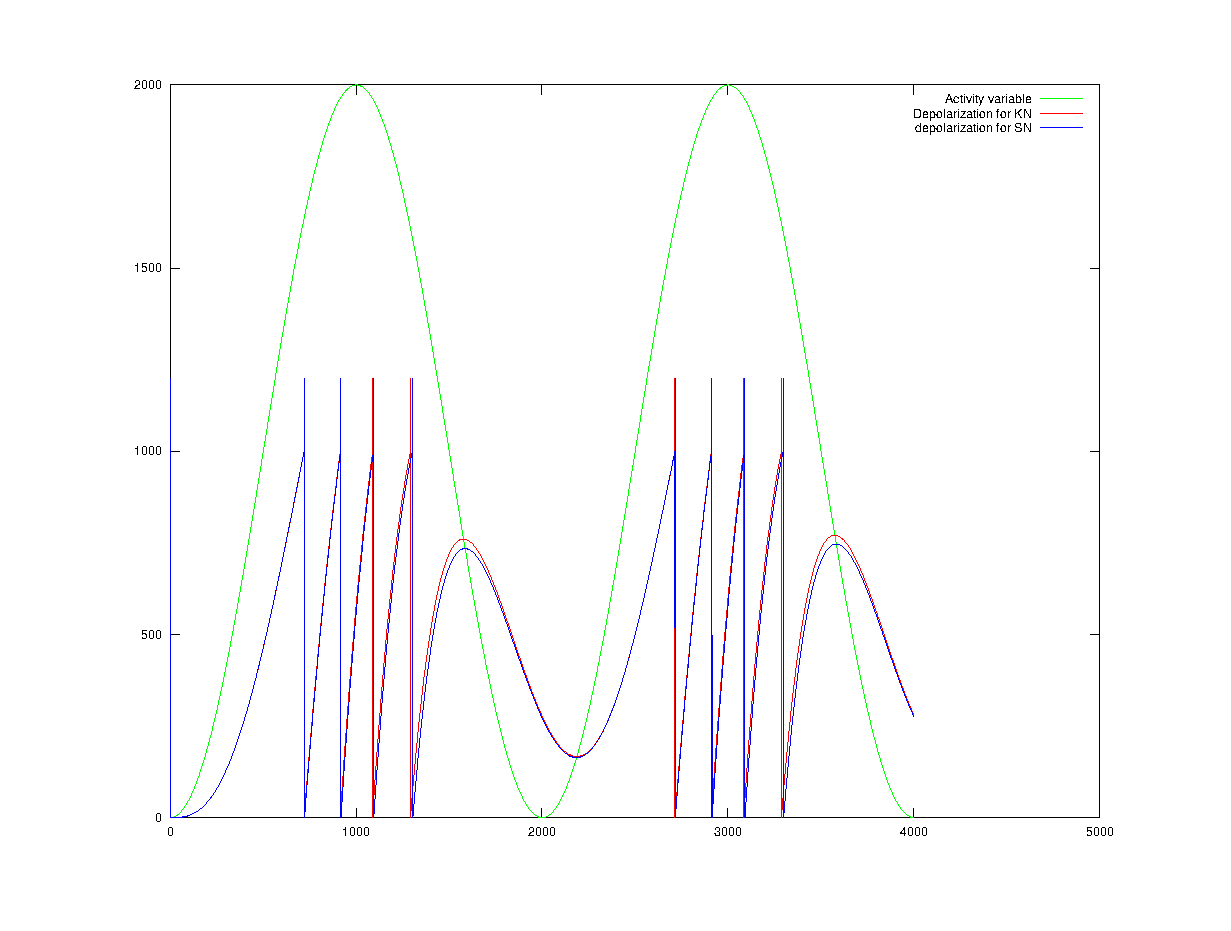
\includegraphics[width=0.95\textwidth]{eps_Comparison_between_the_two_sensors__depol.eps}
	%\end{center}
	\caption{The depolarization curve for a SANN node and a $\kappa$ANN node with the same input. The sensor function is also plotted in green for analysis of the nodes' ``depolarization''. % value. 
	(Generated by AuroSim)}
	\label{figComparisonBetweenSsensorAndKsensorDepolCurve}
\end{figure}

%The sensor function used for the comparison of the time course of the depolarization of a single node is 
The sensor function used in fig. \ref{figComparisonBetweenSsensorAndKsensorDepolCurve} has the formula \mbox{$f(t) = \tau (1 + cos( \frac{\pi \, t}{1000} ))$}, where $\tau$ is the firing threshold for the neuron. 
As defined by in sec. \ref{ssecTheSensorNode}, the activity variable of the K\_sensor\_auron is set to the value of the sensor funciton whenever time is iterated. %every time we iterate time. 
When \emph{time\_class::doTask()} updates the K\_sensor\_auron's activation level, this is done by updating the ``input'' to the dendrite.
% 	%
As can introduced in sec. \ref{ssecTheSensorNode}, this is strongly inspired by the mechanisms of ``receptor cells'' in biology. % Der står: \cite{NeuroscienceExploringTheBrain3edKAP8}. 
%Evt kan eg skrive at "this is strongly inspired by nature".







In figure \ref{figComparisonBetweenSsensorAndKsensorDepolCurve} we can see the results. 
%As can be seen, the depolarization of the K\_auron and the s\_auron is quite simular.
%There is a small difference between the curves.
%It is hard to know the specific reason for the error in this implementation.  In the following section I will discuss possible explanations.
% (Før: linjeskift, her..)
%\subsubsection{Analysis of the difference between the curves}
% SKRIV OM LITT, neste setning: Snakk heller om difference enn om "curve". "Difference" har allerede blitt introduced.
What is interesting about this curve is that it seems that the depolarization curves follow eachother exactly %Dette er rett stavemåte: exactly (google translate)
for the rising phase of the sensor curve. 
For the falling phase of the curve we get a small difference between the depolarization curve of the SN and the $\kappa$N.

% Skrive at for SANN så:
What is the background for the difference between the curves?
For discrete integration we may get something called the trunctation error. 
The ``local truncation error'' is the immediate error after each time step. 
The ``global truncation error'' is the error following integration multiple local truncation errors. 
The global truncation error is defined as the absolute difference between the approximated solution and the actual solution. 
For the SN this might become a problem, and could be the basis of the difference of the simulated node's depolarization.%Skriv om. XXX



%TODO TODO TODO TODO TODO TODO TODO TODO TODO TODO TODO TODO TODO TODO TODO TODO TODO TODO TODO TODO TODO TODO TODO TODO TODO TODO TODO TODO TODO TODO TODO TODO TODO 
%TODO TODO TODO TODO TODO TODO TODO TODO TODO TODO TODO TODO TODO TODO TODO TODO TODO TODO TODO TODO TODO TODO TODO TODO TODO TODO TODO TODO TODO TODO TODO TODO TODO 
%TODO TODO TODO TODO                                                                                                						 TODO TODO TODO TODO TODO 
%TODO TODO TODO TODO                     HER ER EG KOMEN..                                                          						 TODO TODO TODO TODO TODO 
%TODO TODO TODO TODO                                                                                                						 TODO TODO TODO TODO TODO 
%TODO TODO TODO TODO TODO TODO TODO TODO TODO TODO TODO TODO TODO TODO TODO TODO TODO TODO TODO TODO TODO TODO TODO TODO TODO TODO TODO TODO TODO TODO TODO TODO TODO 
%TODO TODO TODO TODO TODO TODO TODO TODO TODO TODO TODO TODO TODO TODO TODO TODO TODO TODO TODO TODO TODO TODO TODO TODO TODO TODO TODO TODO TODO TODO TODO TODO TODO 



	\subsubsection{Trunctation error of the SN} %Kanskje skrive "Spiking Node". Hugs at overskrifta blir også oppført i "index".
	\label{ssecTruncationErrorOfSN}
In SANN each node is modelled as a leaky-integrate-and-fire neuron.
When the depolarization of the SN is updated, the leak of the neuron calculated as the previous value times the leak constant.
The updated value then becomes %todo Skriv om denne setninga.
\begin{equation} %TODO Introduser denne ligninga tidligare i oppgava. Her skal eg bare skrive siste del av den:    v_t = (1-\alpha) * v_{t-1}  XXX HAR EG GJORT DET? TODO SJEKK!
	v_t =  (1-\alpha) \cdot v_{t-1}  
	\label{eqLekkasjeAnalyseAvTruncationError}
\end{equation}
The discretization of time introduces a small error that varies with the size of the time step and the derived of the value function $\dot{v}(t)$.







As the value is updated every time iteration, the leak is calculated by eq. \ref{eqLekkasjeAnalyseAvTruncationError}.
%The leak is implemented by adding $-\alpha v_{t-1}$ to the value $v_t$.
%The leak is calculated as $-\alpha v_{t-1}$.
% Skriv at når feilen oppstår, så er dot(v(t)) positiv, dette gir:
When $\dot{v}(t)$ is positive, $v_{t-1}$ is less than the value $v_t$, varying with the size of the time step and the differentiated value function $\dot{v}(t)$.
When $\dot{v}(t)$ is negative, we get the oposite result.
The resulting leakage will vary correspondingly.
%skriv at dette nuller ut problemet. (MEN (det kommer at) siden det alltid fyrer etter positiv flanke, blir det integral av en liten integralfeil ved kvar fyring. XXX Viktig poeng. Sjekk at det er stort nok skrevet lenger nede.

Each small error is integrated up to a larger error, the global trunction error. 
If some situation is analyzed where the value is the same as the initial value, the integral of the derived over this interval is per definition zero.
The positive contibution will equal the negative contribution, and the trunction error will disappear.
This further implies that for a continous signal that varies around some working point, the global trunctation error will not diverge. 

\begin{figure}[hbt!]
	\centering
	%\begin{center}
		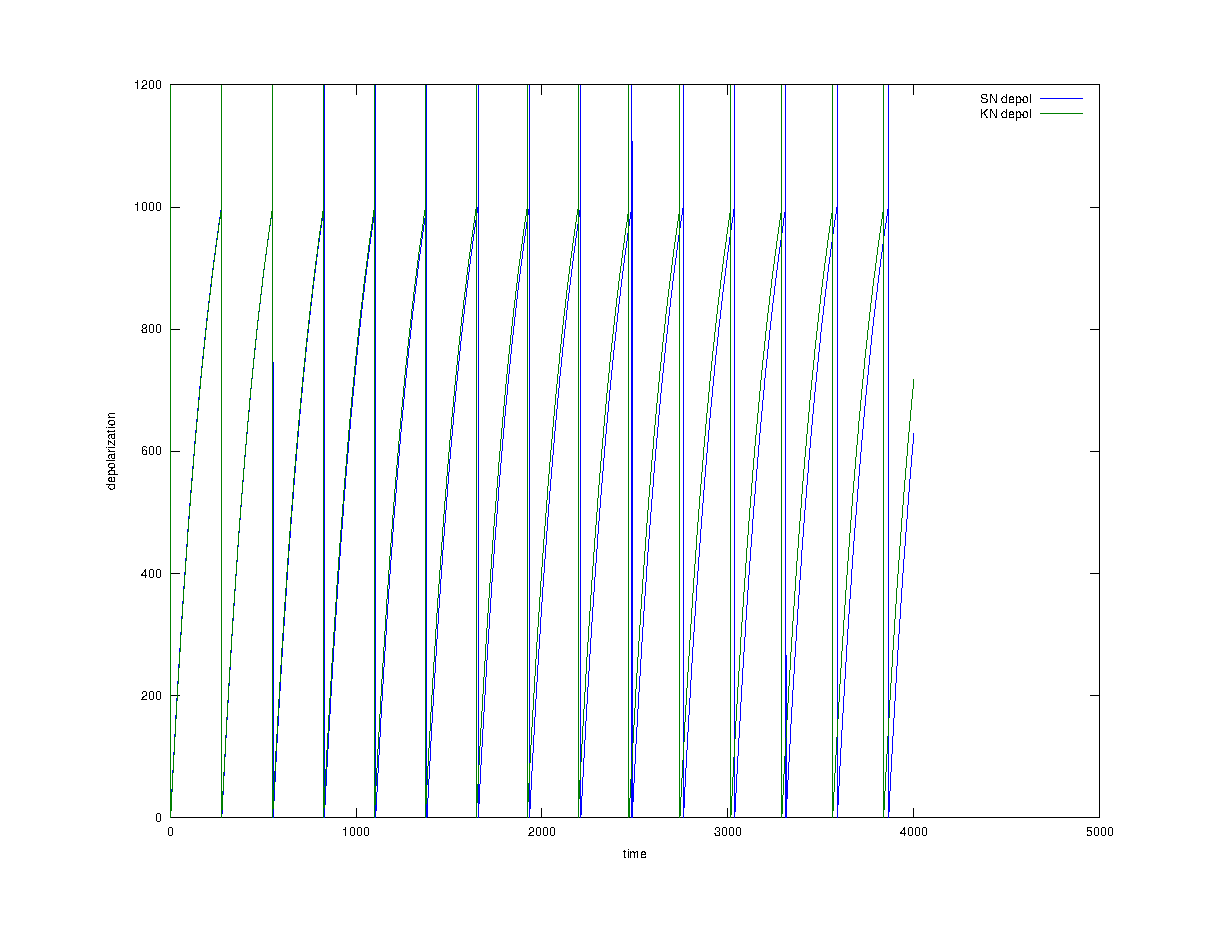
\includegraphics[width=0.95\textwidth]{eps_comparison_between_KN_and_SN_ConstKappa.eps}
	%\end{center}
	\caption{The depolarization curve for a SANN node and a $\kappa$ANN node with the same input. Both sensor nodes have an input that gives an activation level equivalent to $\kappa = 1.5 \tau$ 
			(Generated by AuroSim)} %XXX Eller for begge nodeModeller
	\label{figComparisonBetweenSsensorAndKsensorDepolCurveCONStActivityLevel}
\end{figure}

The depolarization of a neuron have a discontinuity when the neuron fires an action potential. 
When the neurons depolarization reaches the firing threshold the value is reset to $v_0 = 0$.
This gives that we can have a rising phase of indefininite length.
%In other words, each time the value of a node reaches a positive threshold, the value is reset.
We get that the global trunctation error will continue to grow, and that the difference between the value curves for the SN and the $\kappa$N continues to grow.
%In this case the global trunctation error will continue to grow, and the difference between the value curves for the SN and the $\kappa$N continues to grow. %TODO Ikkje dette. Skriv heller eit utfall som Stavdahl vil syns er SKUMMELT!

To see if this is the backgound for the error, we isolate the error by giving the sensor aurons a constant sensor function, with an activation level corresponding to $\kappa = 1.5 \tau$.

The result is presented in fig. \ref{figComparisonBetweenSsensorAndKsensorDepolCurveCONStActivityLevel}. % .eps
It can be observed that the difference between the two curves continues to grow.
If the previous analysis of the problem is sound, the SN should have a depolarization that is higher than is should be.
This implies than the depolarization curve for the SN would be ``before'' that of the $\kappa$N.
A close examination of fig. \ref{figComparisonBetweenSsensorAndKsensorDepolCurveCONStActivityLevel} tells us that this is the opposite of the situation in this experiment.



	\subsubsection{Rounding errors}
%TODO Skriv om: Ikkje røp løysing først. La det være litt spenning!
After an extensive analysis of this error, it was found that the difference comes from a rounding error.
%After a more thorough analysis of the error, it seems that the difference is an effect of a rounding error.

If the error is analyzed with respect to the timing of the curves, it can be observed that the $\kappa$N's depolarization curve lies before the SN's depolarization curve.
%If we change wievpoint on the error and see the difference between the two cuves as an effect of time, we can say that the $\kappa$N's depolarization curve lies before the SN's depolarization curve.
It could be concluded that the $\kappa$N fires before the SN, and thus starts the next period earlier than the SN.
The values of the $\kappa$N would then be a little less than that of the SN.
%This would give the same result as the effect seen in fig. \ref{figComparisonBetweenSsensorAndKsensorDepolCurveCONStActivityLevel}. 
%This implies that the $\kappa$N fires before the SN, and thus starts earlier on the depolarization for the next period.

In many programming languages, a casting from floating point value to an interger causes the value to always be rounded down.

%In many programming languages a float is always ``rounded down''. This means that the DECIMAL %XXX FINN RETT ORD: Det som står etter komma TODO
%	is removed from the number, and the integer becomes the same as the integer part of the number.

%TODO Viktig: Hugs å skrive om kvifor eg valte en mindre periode i starten av sensor-funk. Dette er viktig, ellers trur han nok at eg bruker dette for å skjule feilen..
\begin{figure}[hb!tp]
	\centering
		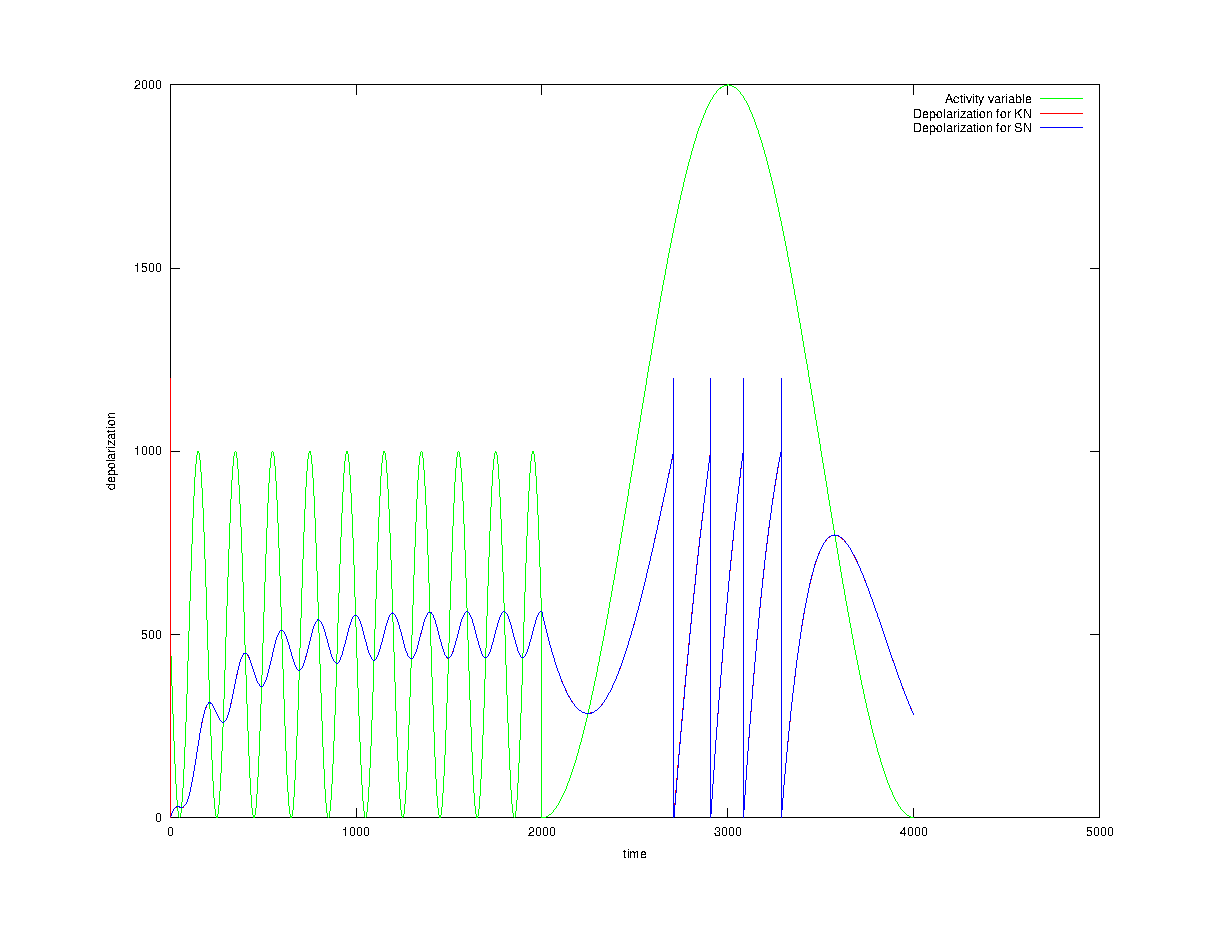
\includegraphics[width=0.95\textwidth]{eps_Comparison_between_the_two_sensors__depol_FIKSA.eps}
	\caption{Comparison between the SN's and $\kappa$N's depolarization curve. The sensor function is plotted in green for analysis purposes. 
			(Generated by AuroSim)}
	\label{figComparisonBetweenSsensorAndKsensorDepolCurveFIXEdError}
\end{figure}

When the $\kappa$N calculates the estimated firing time, this calculation is done in a double precision floating point number. 
%To use this in the scheduler is must first be transformed to an integer variable.
As presented in sec. \ref{secPlannedEvents}, this result has to be casted to an integer variable (\emph{unsigned long ulEstimatedTaskTime\_for\_object}).
%When this time step arrives, the task is executed.

%TODO Skriv at vi vil heller runde til nermeste integer, opp om det er best.
% Så skriv korleis dette gjøres, så finn rett kurve.
% TODO analyser frem og tilbake om kor feilen ligger. Det er fortsatt mulig at feilen er for KANN (men trur ikkje det. Legg at feilen er maks når subthreshold polarization er størst. Osv.) XXX
If this is the effect behind the difference, the error could be fixed by rounding to the ``right'' integer by adding $0.5$ before it is converted into integer.
This vould give a better estimation of the firing time.
The resulting depolarization curve is presented in fig. \ref{figComparisonBetweenSsensorAndKsensorDepolCurveFIXEdError}.
%If we instead round to the closest integer, by adding $0.5$ to the float before it is converted into an integer, we get the depolarization curve presented in fig. \ref{figComparisonBetweenSsensorAndKsensorDepolCurveFIXEdError}.
%In the improved depolarization curves for the auron, the error is small and can not be seen on the plot.
The error is so small that a close examination of a vetor graphics variant of the plot is needed to observe any difference between the two.

%Ikkje heilt sikker på om det er heilt rett: størst etter "rising flank of the ..", Bli heilt sikker på dette.
The error can not be seen in the plot presented in fig. \ref{figComparisonBetweenSsensorAndKsensorDepolCurveFIXEdError}, and to compare the two it was nessecary to read the values directly from the octave log files.
%To compare the difference between the curve, a direct comparison of the values in the two log files was carried out.
The error was found to be largest right after the rising flank of the curves, at time $t=3000$. 
The comparison of the two log files showed that the SN was $1.015$ larger than the value of the $\kappa$N at this time.
For a situation where the firing threshold is $\tau=1000$, an error of size $1.015$ does not matter much, but this was only after a simulation of four seconds (4000 iterations). 
%Examination of the values listed in the \emph{.oct} log files created by AuroSim, this error is greatest at time step number $3000$.
%The SN is $1.015$ more than the value of the $\kappa$N.
We can, however, conclude that the error behaves exactly like predicted in the analysis of a possible trunctation error.
%This is an error that behaves like the analysis of a truncation error.
%At this time iteration the value of the SN is 1.015 more than the value of the $\kappa$N. 

The deviation caused by the trunctation error is very small for a simulation of this lenght.
%The deviation is substantially smaller than the deviation caused by the rounding error.
This discussion is still included in this report, as it shows one aspect that could create large errors for neural simulation. 
When the aspect of global truncation error is combined with a systematic non--continuity, where the value of a node is reset after firing, the error grows larger.
The error now becomes the sum of all the global truncation errors from all periods, or the integral of the integral of the local truncation error.
This could give errors of a considerable size. 

%The error could grow large when the aspect of a global truncation error is combined with a systematic non--continuity that resets the value after a sufficient rising phase. % (reset to zero after a sufficient rising phase

% //{ Her er historia om korleis eg fann feilen:
% - integralfeil for SN
% - Integralfeilen kommer antagelig av at lekkasjen  
% - For SN vil lekkasjen regnes ut fra verdien ved forrige tissteg. Denne diskretiseringseffekten vil forplante seg i at for positiv derivert av depol-kurva vil SN-depol være litt over, og for negativ flanke : motsatt.
% 		Dette er fordi lekkasjen regnes ut fra forrige verdi, som for stigende flanke er mindre enn den noværande verdien, og vi får en mindre lekkasje => for stor verdi.
% - denne feilen vil nulles ut for eit periodisk signal uten sprang (over en periode vil integralet av positiv flanke og neg. flanke bli null.
% - dersom vi har eit sprang, eller enda verre: eit sprang som alltid ligger etter en viss mengde med pos. flanke, vil vi få summert opp integral-feilen.
% For auronet vil depol settes lik 0 etter en viss mendge pos. flanke for depol. kurva. Dette skaper problemet.

% Eg har også vurdert om det er feil fra implemenasjonen: at de har ulik refraction time, MEN eg trur ikkje dette: 
% 		En slik feil ville vore mindre (eit-to tidssteg per fyring) => ikkje synlig på eit plott over fleire tusen iter's.

% ROUNDING ERROR!

% Den lille forskjellen mellom s_sensor_auron og K_sensor_auron er noko eg kan skrive mykje om i 'discussion'.
% Eg har tanker om at det er pga. at eg bruker integer (tid) i ligningene, og vi får dermed avrundingsfeil. Litt overraska over at feilen er så liten..
% 	Det er også mulig at den lille forskjellen kommer av forskellane i korleis sensor-funksjonen blir oversatt til depol.
% 		- K_sensor_auron oversetter sensorFunk direkte til aktivitetsVariabel Kappa, mens
% 		- s_sensor_auron sender gir eit enkelt input per tidsiterasjon gitt av ligninga (W_ij / [time constant]), eller  ALPHA * W_ij
%   XXX Dette trenger grundigare analyser!

% Svaret var: avrundingsfeil av casting fra float til unsigned (fra estimering av tidssteg til Tidssteg). Dette ble alltid runda ned. Løste ved å +0.5 før casting. Funker drita bra!
% //}









	\subsection{Analysis of Synaptic Transmission as the derived}
			%\subsection{Analysis of synaptic transmission as the derived}
			\label{ssecAnalysisOfSynTransAsTheDerived}
			To avoid summation of all the node's synaptic input every time one is updated, the concept of the edge transmission as the derives was introduced
			%To avoid summation of the transmission of all node's input synapses, the edge transmission is defined as the derived.
			%
			%To update the synapse's $\kappa_{ij}$, the edge transmission only has to be added to the previous $\kappa_{ij}$. %ta med?  :   that is the change of the synapse's transmission   før "only"?
			%As a node's activity variable $\kappa_i$ is defined as the sum of all the input transmissions, $\kappa_{ij}$,
			%	the postsynaptic activity variable is also updated by summing it with the new edge transmission.
			By the use of this aspect in $\kappa$ANN, updating the postsynaptic $\kappa$ after an edge transmission is trivial.
			% is done by simply adding the edge transmission to the current value of $\kappa$.
	
			After each transmission, $\kappa_i$ is updated by adding the edge transmission $u_{ij}(\kappa_j)$. 	 	 % to the current $\kappa_i$.
			\begin{equation}
				\kappa_{i, new} = \kappa_{i} + u_{ij}(\kappa_j)
			\end{equation}
			
			%xxx BRA SETN.:  As the effect of synaptic transmission first gets calculated after the current time iteration, further propagation of the signal happens at the next time iteration.
			
			
			In fig. \ref{figEdgeTransmissionKaboveT} we can see a plot of the edge transmission of an \emph{inhibitory} synapse.
			The presynaptic node is a sensor function, with a sensor funtion \mbox{$f(t) = 1.1 \cdot \tau \cdot (2 + sin( 2\pi \cdot \frac{t}{1000})$}.
			The activity level $\kappa_{pre}$ is plotted in blue and the edge transmission in red.
			%The presynaptic node's activity variable varies as \mbox{$f(t) = 1.1 \cdot \tau \cdot (1 + sin( 2\pi \cdot \frac{t}{1000})$}.
	
\begin{figure}[hb!tp]
	\centering
	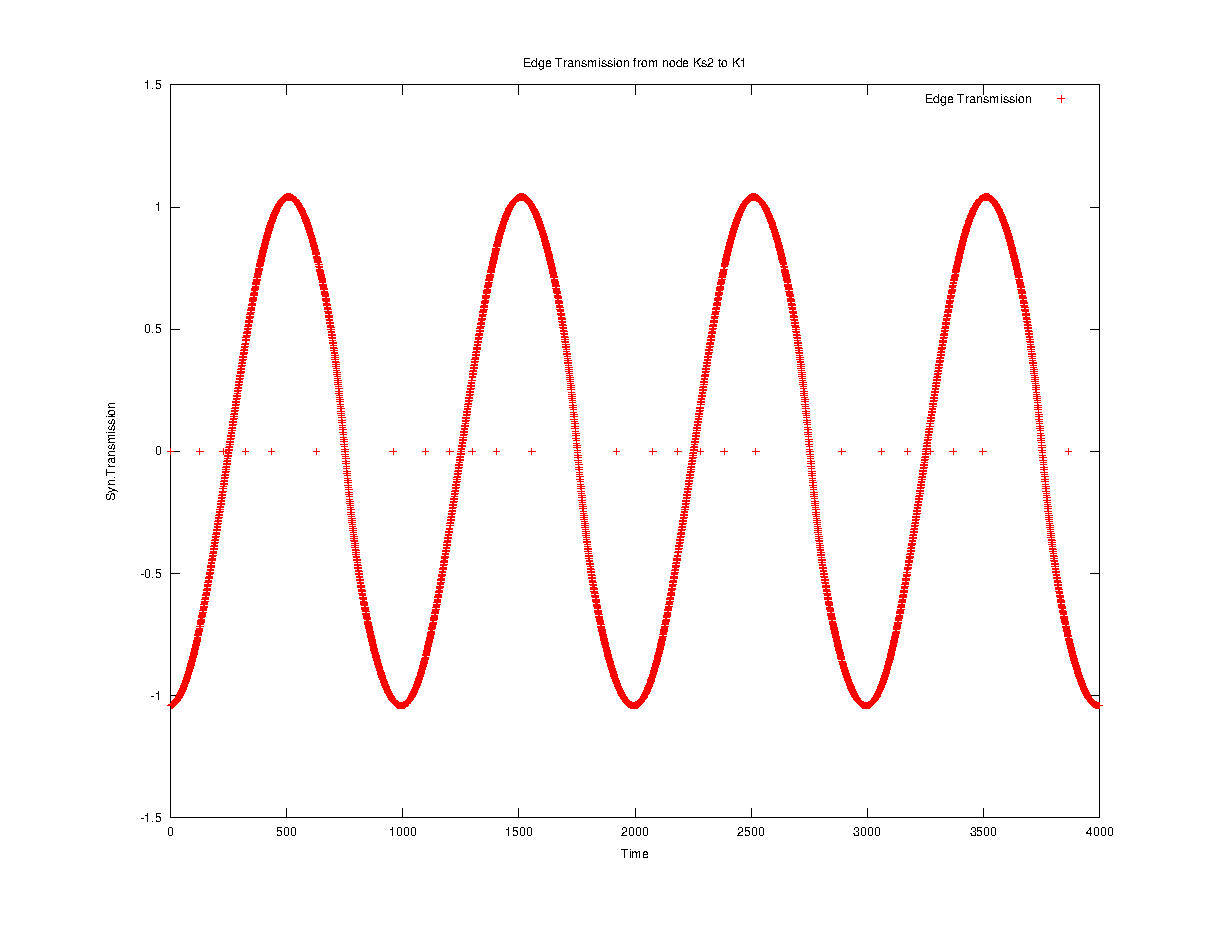
\includegraphics[width=0.95\textwidth]{./synapticTransmissionPlots/eps_transmissionKappaAboveThreshold.eps} 	
	\caption{Synaptic transmission for a synapse with a presynaptic sensor funciton \mbox{$f(t) = 1.1 \cdot \tau \cdot (1 + sin( 2\pi \cdot \frac{t}{1000})$}. 
			Notice that for this analysis, the sensor fuction will allways be larger than the firing threshold (curve is scaled by $\frac{1}{\tau}$ to fit). \\
			(Edge transmission is generated by AuroSim)} 
	\label{figEdgeTransmissionKaboveT}
\end{figure}

			The edge transmission for an inhibitory synapse causes an inhibition of the postsynaptic node, and is negative of the transmission of an excitatory synapse.
			%The edge transmission for an inhibitory synapse is the negative of that of an excitatory synapse.
			As the time resolution in the sensor function is defined to 1000 iterations, the change each time step is given by $\frac{\Delta f(t)}{1000 \Delta t}$
			This explains the amplitude of the curve for synaptic transmission as $1.1 = \frac{1100}{1000}$
%			The sensor function is given as $f(t) = 1100 \cdot (1+ sin(2 \pi \frac{t}{1000}))$.
%			We get that the synaptic transmission is the derived of the sensor function devided by 1000.
%			\begin{equation}
%				u_{ij}(t) = \frac{\Delta f(t)}{1000} = 1100 \cdot \left(1+ sin\left(2 \pi \frac{t_n-t_{n-1} }{1000}\right) \right)
%			\end{equation}

			We can further see that the curve in fig. \ref{figEdgeTransmissionKaboveT} resembles that of the function $g(x)= - 1.1 \cdot cos(x)$. 
			From this we can assume that for the implementation, we have that
			\begin{itemize}
				\item[a)] Edge transmission is the derived of the presynaptic $\kappa$, scaled by the time resolution.
				\item[b)] Inhibitory synaptic transmission gives a negative synaptic transmission.
			\end{itemize}
			As this is apects that follow the definitions for synaptic transmission in $\kappa$ANN (see sec. \ref{ssecSynTransForANNliggeriKANNsection} and \ref{ssecSynInputToANodeKANN})
				, we can conclude that the impelementation works as designed.
			Is should be emphasised that the synapse is an inhibitory synapse, and this is the reason for the plot of the edge transmissions is the negative of the derived of the presynaptic activity level.

\begin{figure}[hbt!p] 
	\centering
	%
   	\subfloat[Presynaptic activity variable, {$\kappa_j$}]{\label{figEdgeTransmission:edge-a} 						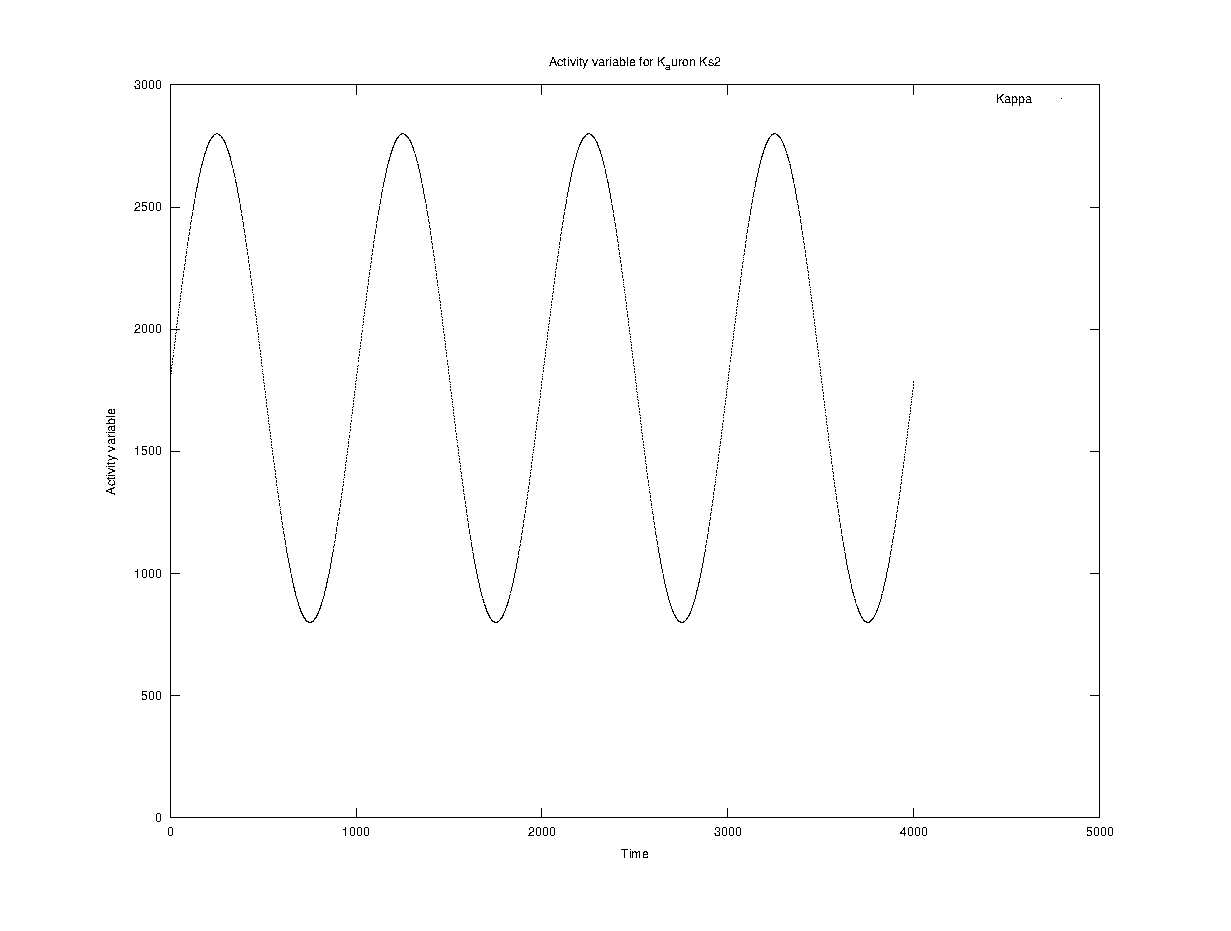
\includegraphics[width=0.95\textwidth]{./synapticTransmissionPlots/eps_auronKs2-kappa.eps} 		}  \\
   	\subfloat[Synaptic transmission]{\label{figEdgeTransmission:edge-b} 		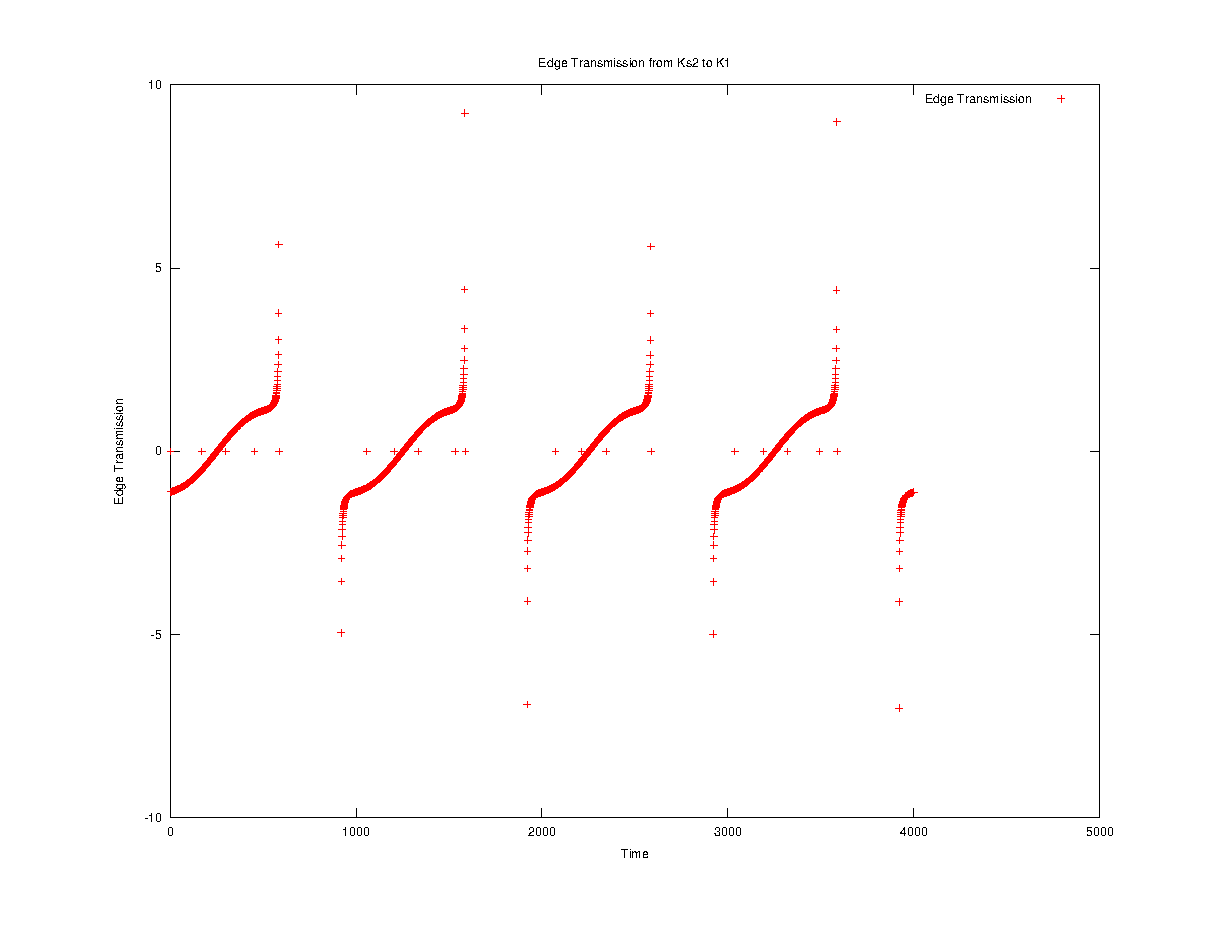
\includegraphics[width=0.95\textwidth]{./synapticTransmissionPlots/eps_transmission_Ks2->K1.eps} 	}
	%\caption{Demonstration of the value function for changing kappa}
	\caption{ 	( \ref{figEdgeTransmission:edge-a} ) The presynaptic activity variable $\kappa_j$         and   
				( \ref{figEdgeTransmission:edge-b} ) The corresponding edge transmission to a presynaptic activity variable presented in \ref{figEdgeTransmission:edge-a}. 
			Notice the gap of the synaptic transmission when $\kappa_j \leq \tau$ = 1000.  
			(Generated by AuroSim)
			} %TODO skriv om dette tomrommet i teksten under.
	\label{figEdgeTransmission}
\end{figure}
			


		%	If we let the presynaptic activity variable ``dip'' below threshold, the \emph{synaptic} transmission becomes zero,
		%	If we let the presynaptic activity variable ``dip'' below threshold, the node will never fire, and the \emph{synaptic} transmission becomes zero.
	%			the \emph{synaptic} transmission becomes zero
	%		 	as the the node never will fire for a sub--threshold activity variable. 
			If we let the presynaptic activity variable ``dip'' below threshold, the node will never fire.
			This causes the \emph{synaptic} transmission $\kappa_{ij} = 0$.
		%
		%	As the synaptic transmission is defined as the synaptic weight times the inverse of the period, the synaptic transmission is zero when $\kappa$ is less than $\tau$.
			This gives a non--continuity for the derived, and causes the artifacts observed in fig. \ref{figEdgeTransmission}. 
			%Combined with the concept of the edge transmission as the derived of the synaptic transmission is what causes in the artifacts in fig. \ref{figEdgeTransmission}. 
			%For the edge transmission we therefore see the strange behaviour in fig. \ref{figEdgeTransmission:edge-b} when the activity variable becomes less than or equal to the threshold. %XXX Skriv om. 

	% Feil ref.		The presynaptic node's activity variable is presented in fig. \ref{figEdgeTransmission:edge-a}.

			Let the sensor function of the presynaptic node be a sinusiodal function that ``dips'' below threshold, as presented in fig. \ref{figEdgeTransmission:edge-a}.
			We can see the resulting edge transmission in \ref{figEdgeTransmission:edge-b}.
			%If the presynaptic node is a sensor neuron with a sensor function varying as a sinus that dips below threshold, we get the edge transmission presented in fig. \ref{figEdgeTransmission:edge-b}. 
			%The presynaptic activity variable is presented in fig. \ref{figEdgeTransmission:edge-a}.
% 	% 	% 	%
			The edge transmission no longer resembles the derived of the presynaptic activity function.
			As discussed, the non--continuity introduced by the presynaptic activity variable going below firing threshold gives the ``pause'' in edge transmission.
			During the pause, the edge transmission is zero, but transmission of zero has been optimalized away.
			The plot thus only shows the pause in transmission when $\kappa_j \leq \tau$.


			We can see that the edge transmission no longer resembles the derived of the presynaptic activity function. 
			We now have a strong non--continuity when $\kappa_j \leq \tau$.
			In all examples in this report, the firing threshold is set to $1000$.







%TODO Flytte analyse over, over til comparison and  results? nee..
%TODO synaptisk transmission overføringsplott, som viser pre og postsyn aktivitetsvar.? Eit som ikkje har problemer: for å vise at det funker..







	%\subsection{Analysis of the postsynaptic activity variable as a result of syn. transmission} % KANSKJE
	\subsection{etc.}


